\documentclass{article}  % 选择模版,这里是使用Latex自带的article模版
    \author{Hongyu Chen}
    \title{CSC 311 - Assignment 2}
    \usepackage{graphicx}   % 插入图片用到的宏包
\begin{document} 
    \maketitle
   \section{4. Neural Networks: theory} 

        \subsection{4a)} 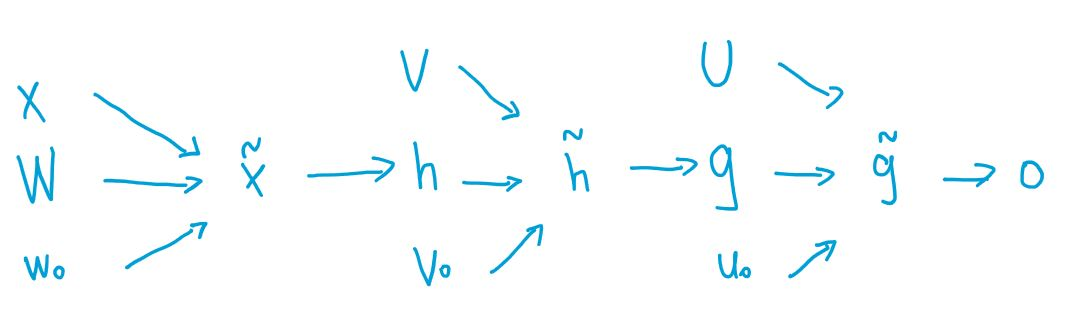
\includegraphics[width=0.90\textwidth]{./4a.JPG} 
		 \subsection{4b)}
		 We first prove that:\\\\
		 $\frac{\partial(c(t,o))}{\partial\tilde{g}_{j}} 
		 = \frac{\partial (-tlogo-(1-t)log(1-o))}{\partial\tilde{g}_{j}}$    (by equation (9)) \\\\
		 $= -t \frac{logo}{\partial\tilde{g}_{j}} - (1-t)\frac{log(1-o)}{\partial\tilde{g}_{j}}$		  (Since t is a binary value which is a constant)\\\\
		 $ = -\frac{t}{o}\frac{\partial o}{\partial\tilde{g}_{j}} - \frac{1-t}{1-o}\frac{\partial(1-o)}{\partial\tilde{g}_{j}}$ (By chain rule)\\\\
		 $ = -\frac{t_{j}}{o_{j}}(o_{j}(1-o_{j})) + \frac{1-t_{j}}{1-o_{j}}(o_{j}(1-o_{j}))$ (by equation (8) $o_{j} = \sigma(\tilde{g_{j}}))$\\\\
		 $ = -t_{j}(1-o_{j}) + (1-t_{j})o_{j} \\\\ = -t_{j} + t_{j}o_{j} + o_{j} - o_{j}t_{j} \\\\ = o_{j}-t_{j}$\\\\
		 Then:\\\\
		 $[\frac{\partial C}{\partial \tilde{G}}]_{nj} $ 
		 $= \frac{\partial C}{\partial \tilde{G}_{nj}}$ 
		 $= \frac{\partial C}{\partial \tilde{g}^{(n)}_{j}}$ (by definition of gradient)\\\\

		 $=\frac{\partial(c(t^{(n)},o^{(n)}))}{\partial\tilde{g}^{(n)}_{j}}$ (by equation (9) and we only care about $o^n$ here since it's depends on $\tilde{g}^{(n)}_{j}$)\\\\
		 = $  o_{j}^{(n)}-t_{j}^{(n)}$ (by the prove above)\\\\
		 = $ O_{nj} - T_{nj} = [O-T]_{nj}$\\\\
		 Which means all of their components are equal to each other. So
		  $\frac{\partial C}{\partial \tilde{G}} = O-T$
		  
		 \subsection{4c)}
		 $[\frac{\partial C}{\partial \tilde{H}}]_{nk} = 
		 \frac{\partial C}{\partial \tilde{H}_{nk}}$ (by definition of gradient)\\\\
		 $ = \frac{\partial C}{\partial \tilde{h}^{(n)}_{k}} $  \\\\
		 $ = \frac{\partial C}{\partial g^{(n)}_{k}} \frac{\partial g_{k}^{(n)}}{\partial \tilde{h}_{k}^{(n)}}$ (by chain rule)\\\\
		 $=\frac{\partial C}{\partial g^{(n)}_{k}} (1 - (g^{(n)}_{k})^2)$ (By equation (7) $g = tanh(\tilde{h})$ (equation 5))\\\\
		 $ = \frac{\partial C}{\partial G_{nk}} (1 - (G_{nk})^2)$\\\\
		 $= (1-G^2_{nk})[\frac{\partial C}{\partial G}]_{nk}
$
		\subsection{4d)}
		First we need to know:\\\\
		 $[\frac{\partial C}{\partial \tilde{H}}]_{nj} $ 
		 $= \frac{\partial C}{\partial \tilde{H}_{nj}}$ 
		 $= \frac{\partial C}{\partial \tilde{h}^{(n)}_{j}}$ (by definition of gradient)\\\\
		 $= \frac{\partial \sum_{m} c(t^{m},o^{m})}{\partial \tilde{h}^{(n)}_{j}}$ (by equation (9))\\\\
		 $=\frac{\partial(c(t^{(n)},o^{(n)}))}{\partial\tilde{h}^{(n)}_{j}}$ (we only care about $o^n$ here since it's depends on $\tilde{h}^{(n)}_{j}$)\\\\
		 Then:\\\\
		 $[\frac{\partial C}{\partial V}]_{kj} =  \frac{\partial C}{\partial V_{kj}}$\\\\
		 $= \frac{\partial \sum_{n} c(t^{(n)},o^{(n)})}{\partial V_{kj}}$ (by equation (9))\\\\		$ = \sum_{n}\frac{\partial c(t^{(n)},o^{(n)})}{\partial V_{kj}}$\\\\
		 $ = \sum_{n}\frac{\partial c(t^{(n)},o^{(n)})}{\partial \tilde{h}_{j}^{(n)}}
		 \frac{\partial \tilde{h}_{j}^{(n)}}{\partial V_{kj}}$ (by chain rule)\\\\
		 $ =  \sum_{n}[\frac{\partial C}{\partial \tilde{H}}]_{nj}\frac{\partial \tilde{h}_{j}^{(n)}}{\partial V_{kj}}$ (by the prove about)\\\\
		 (By equation (5) we know that $\tilde{h} = hV + v_{0}$ so :\\\\
		 $\frac{\partial \tilde{h}_{j}^{(n)}}{\partial V_{kj}}$
		 $=h_{k}^{(n)}$)\\\\
		 So we continue the calculation from above:\\\\
		 $ =  \sum_{n}[\frac{\partial C}{\partial \tilde{H}}]_{nj}h_{k}^{(n)}$\\\
		 $ =  \sum_{n}[\frac{\partial C}{\partial \tilde{H}}]_{nj}H_{nk}$\\\\\
		 $ =  \sum_{n}[\frac{\partial C}{\partial \tilde{H}}]_{nj}H^{T}_{kn}$\\\\
		 $ =  \sum_{n}[H^{T}]_{kn}[\frac{\partial C}{\partial \tilde{H}}]_{nj}$ (Matrix multiplication)\\\\
		 $ =  [H^T \frac{\partial C}{\partial \tilde{H}}]_{kj}$\\\\
		 Then $\frac{\partial C}{\partial V} = H^T \frac{\partial C}{\partial \tilde{H}}$ Since every components in these two are equal.
		 \subsection{4e)}
		According to the proof from part 4(d) we know that :\\\\
		$[\frac{\partial C}{ v_{0}}]_{j} =  \sum_{n}[\frac{\partial C}{\partial \tilde{H}}]_{nj}\frac{\partial \tilde{h}_{j}^{(n)}}{\partial {v_{0}}_{j}} $\\\\
		$ = \sum_{n}[\frac{\partial C}{\partial \tilde{H}}]_{nj} \vec{1}$ (By equation 5 ,$v_{0}$ is a constant)\\\\
		$ = \sum_{n}[\vec{1}]_{n}[\frac{\partial C}{\partial \tilde{H}}]_{nj}$\\\\
		$ = [\vec{1}\frac{\partial C}{\partial \tilde{H}}]_{j}$ (By matrix multiplication)\\\\
		Then we know that $\frac{\partial C}{\partial v_{0}} = \vec{1} \frac{\partial C}{\partial \tilde{H}}$ Since every components in these two are equal.
		 \subsection{4f)}
		 $[\frac{\partial C}{\partial H}]_{nk} $ 
		 $= \frac{\partial C}{\partial H_{nk}}$ 
		 $= \frac{\partial C}{\partial h^{(n)}_{k}}$ (by definition of gradient)\\\\
		 $= \frac{\partial \sum_{m} c(t^{m},o^{m})}{\partial h^{(n)}_{k}}$ (by equation (9))\\\\
		 $=\frac{\partial(c(t^{(n)},o^{(n)}))}{\partial h^{(n)}_{k}}$ (we only care about $o^n$ here since it's depends on $h^{(n)}_{k}$)\\\\
		 $ = \sum_{j} \frac{\partial(c(t^{(n)},o^{(n)}))}{\partial \tilde{h}_{j}^{n}}\frac{\partial \tilde{h}_{j}^{n}}{\partial h^{(n)}_{k}}$ (By equation (10))\\\\
		 $ = \sum_{j} [\frac{\partial C}{\partial \tilde{H}}]_{nj} \frac{\partial \tilde{h}_{j}^{n}}{\partial h^{(n)}_{k}} $ (By the first part proof of 4d))\\\\
		 $=\sum_{j} [\frac{\partial C}{\partial \tilde{H}}]_{nj} V_{kj}$ (By equation (5))\\\\
		 $= \sum_{j} [\frac{\partial C}{\partial \tilde{H}}]_{nj} V^{T}_{jk}$\\\\
		 $= [\frac{\partial C}{\partial \tilde{H}}V^{T}]_{nk}$ (By matrix multiplication)\\\\
		 Then we know that $\frac{\partial C}{\partial H} = \frac{\partial C}{\partial \tilde{H}} V^{T}$ Since every components in these two are equal.
\section{5. Neural Networks: implementation}
 \subsection{5e)} 
 In this question we set the maximum number of iteration as 1. The reason for accuracy decreases with batch size, and cross entropy increases is for small batch size, the learning process will converges very quickly, but for the large batch size, the learning process will converge slowly. At the same iteration smaller batch size will converge faster. Here is the run time for each iteration of my program:\\\\
 batch size (2**0) runtime: 23.266368627548218\\
batch size (2**1) runtime: 11.932782173156738\\
batch size (2**2) runtime: 5.774262189865112\\
batch size (2**3) runtime: 3.154838800430298\\
batch size (2**4) runtime: 1.7582886219024658\\
batch size (2**5) runtime: 1.2529397010803223\\
batch size (2**6) runtime: 0.8675491809844971\\
batch size (2**7) runtime: 0.6975538730621338\\
batch size (2**8) runtime: 0.5969803333282471\\
batch size (2**9) runtime: 0.5671384334564209\\
batch size (2**10) runtime: 0.5290675163269043\\
batch size (2**11) runtime: 0.5251491069793701\\
batch size (2**12) runtime: 0.5324108600616455\\
batch size (2**13) runtime: 0.5390825271606445\\\\
Using batch size of 1 is inefficient. The run time of using batch size 1 is very high. If we want to execute the program on a massively parallel machine, such as a gpu with batch size of 1, it will take a really long run time. GPUs are not inefficient for small batch sizes
\end{document} 